\title{Developing a Robust Algorithm to\\Measure Geometric Distortion in MRIs}
\author{
J. David Giese\\
Innolitics, LLC\\
\and
Yujan Shrestha, M.D.\\
Innolitics, LLC\\
}
\date{\today}

\documentclass[12pt]{article}

\usepackage{amsmath, amssymb, amsbsy}
\usepackage{cite, graphicx}
\usepackage{subcaption}
\usepackage[font={footnotesize}]{caption}

\begin{document}
\maketitle

\section*{Introduction}
MR scanners can introduce geometric distortion into their images.  For many applications these small distortions are not clinically relevant---for others they are relevant and worth measuring and correcting.  A detailed discussion of the causes of geometric distortion in MRIs and the applications in which they matter is beyond the scope of this report, however, there are good articles that cover these topics \cite{baldwin2007,torfeh2015,wang2005,mribook}.  

This report presents the steps we have taken towards developing a robust algorithm to measure geometric distortion introduced by MR scanners using images of grid phantoms.  Our algorithm calculate the geometric distortion from these phantom images using the displacement of fiducials from their known locations.

The first section of this report presents a representation of the problem our algorithm is solving.  It includes several assumptions we make about the phantom images.  The second section presents an overview of our algorithm.  The third section outlines a system for testing the algorithm, and includes preliminary results.  The final section discusses the limitations of our algorithm and directions for future improvements.

\section*{Problem}
Calculating a scanner's geometric distortion from a grid phantom image is a fiducial-based non-rigid registration problem \cite{hill2001}.  We are registering an image of the phantom containing geometric distortion with an image of the phantom that does not contain geometric distortion using the grid intersections as fiducials.

The registration produces a transformation which maps locations in the first image to locations in the second.  This transformation will contain a rigid component (i.e. translation and rotation) and a non-rigid component.  The rigid component is assumed to originate from misalignment of the phantom within the scanner.  The non-rigid component is a measurement of the geometric distortion.

The distortionless image can be a CT of the phantom---where we assume that the CT does not introduce its own geometric distortion---or, if we are willing to neglect phantom manufacturing errors, it can be derived from knowledge of the phantom's design.

Generic non-rigid registration is an open research area with many unsolved problems.  Fortunately we can make several assumptions which make the problem tractable.

We assume that the phantom has set of consistently oriented and formed features that can act as fiducials.  A phantom that contains a Cartesian grid of intersecting cylindrical rods---our typical use case---satisfies this assumption.

We assume that we know the fiducial locations in the undistorted image.  (In the context of Figure \ref{fig:problem-overview}e we would know the square locations.)  This assumption is satisfied because we can derive the undistorted fiducial locations from the phantom's design.  If we wanted to use a CT, we could first detect its features using the theoretical locations, and then in turn use the CT fiducial locations against the MRI.

We assume the images are sufficiently resolved such that the phantom grid fiducials are detectable.  In the case of a phantom with cylindrical grid intersections, this means that the pixel spacing along all three dimensions is larger than the intersecting rods.

We assume that the scanner introduces minimal geometric distortion near its isocenter.  This assumption may be more or less valid for certain scan parameters.  For example, automatic shimming will increase the homogeneity of the static magnet near the isocenter, but this setting can be turned off \cite{baldwin2007}.

Finally, we assume that the images are crudely registered.  In particular, we assume that the magnitude of the translation component of the registration is less than the phantom grid spacing.  We also assume that the rotation component is less than a few degrees.  Our algorithm could be improved so as to not require this assumption.

Figure \ref{fig:problem-overview} demonstrates the registration process with an example image.  Figure \ref{fig:generic-algorithm} is a block diagram of the generic algorithm, taking into account our assumption that we know the fiducial locations in the undistorted image.

\begin{figure}[h]
    \centering
    \includegraphics[width=\linewidth]{problem-overview.pdf}
    \caption{The geometric distortion is measured using a non-rigid registration. \textbf{(a)} An image of a ``phantom'' without any distortion.  In practice this could be a CT or an image derived from a CAD model of the phantom.  \textbf{(b)} A distorted image of the phantom---for example, an MRI of the phantom.  \textbf{(c)} The images (a) and (b) overlaid without any registration.  \textbf{(d)} A rigid registration is applied to (b) and then overlaid on (a).  The rigid registration cancels out any alignment errors that were introduced when the phantom was positioned in the scanner. \textbf{(e)} A detail of (d) highlighting the displacement between fiducials in the undistorted image (squares) and the fiducials in the distorted image (circles).  The remaining distortion between the two images would be corrected by a full non-rigid registration. \textbf{(f)} The geometric distortion can be interpolated from the non-rigid component of the registration.}
    \label{fig:problem-overview}
\end{figure}

\begin{figure}[h!]
    \centering
    \includegraphics[width=\linewidth]{generic-algorithm.pdf}
    \caption{A generic representation of the problem we are solving. We assume that we know the fiducial locations in the undistorted image.  Our algorithm must apply a rigid registration to remove alignment errors (see Figure \ref{fig:problem-overview}d) and return the locations of the registered fiducials.  These registered fiducials can be used to interpolate the geometric distortion vector field.}
    \label{fig:generic-algorithm}
\end{figure}


\section*{Solution}
We have developed a feature detection and rigid-registration algorithm that can be used to detect geometric distortion in MRIs.  Developing an algorithm that works on a particular image has been straightforward.  Developing an algorithm that works on a large variety of images is likely to be more difficult.

Adjustments that improve an algorithm's performance on a particular image often degrade its performance on others.  For this reason, instead of spending too much effort optimizing our algorithm's performance on a particular image, we have built a testing system that allows us to quickly validate an algorithms against many images.  As we collect more datasets from early customers and beta-testers, we can use this system to further refine our algorithm until it works well on a large variety of phantoms and MRIs.

In the remainder of this section we will present our testing system and provide an overview of our current algorithm.

\subsection*{Testing System}
The final output of our system is a measurement of the geometric distortion vector field introduced by the scanner.  Because we do not know the actual distortion field of a real MRI, we can not directly verify our algorithm.  To work around this limitation, while still using actual MRIs, we apply additional distortion to an MRI.  We call the underlying MRI the ``source image''.  The source image may or may not already have its own distortion, but as you will see, any existing distortion is accounted for and effectively ignored in our testing.

Before we can run our tests, we first manually annotate each fiducial in the source image.  Next we apply a known geometric distortion to the source image, producing a distorted image.  We may also add noise, amplitude fluctuations, rotations, or translations to the distorted image in order to further strain our algorithm.  We can then run our algorithm on the distorted image, using the fiducials captured from the source image, and compare the resulting output.  Our testing process is illustrated in Figure \ref{fig:testing-setup}.

\begin{figure}[h]
    \centering
    \includegraphics[width=\linewidth]{testing-setup.pdf}
    \caption{Overview of our testing setup.  We can quantitatively validate our algorithms using this approach because we know the actual geometric distortion that was applied to the source image.}
    \label{fig:testing-setup}
\end{figure}

Annotating a source image is time consuming.  We tried using existing tools, such as 3DSlicer, however we found them to be too slow and inflexible for our needs.  Thus, we built a simple GUI tool that haw allowed us to quickly annotate images.  We can annotate even a large phantom MRI with thousands of points in about an hour, using our tool.  This is possible because we built various keyboard shortcuts into the GUI that allows us to annotate about one point per second with sufficient accuracy.

Once we have annotated a source image, we can generate many test cases from it by applying various combinations of distortions, rigid registrations, noise, and filters to the original image.  Figure \ref{fig:test-case} demonstrates an example test case with extreme distortion.

\begin{figure}
    \centering
    \begin{subfigure}[b]{0.48\textwidth}
        \centering
        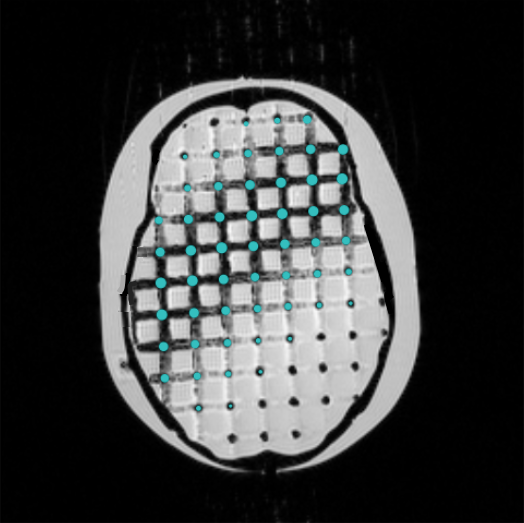
\includegraphics[width=\textwidth]{source-image.png}
        \caption{Source Image}
        \label{fig:test-case_1}
    \end{subfigure}%
    ~
    \begin{subfigure}[b]{0.48\textwidth}
        \centering
        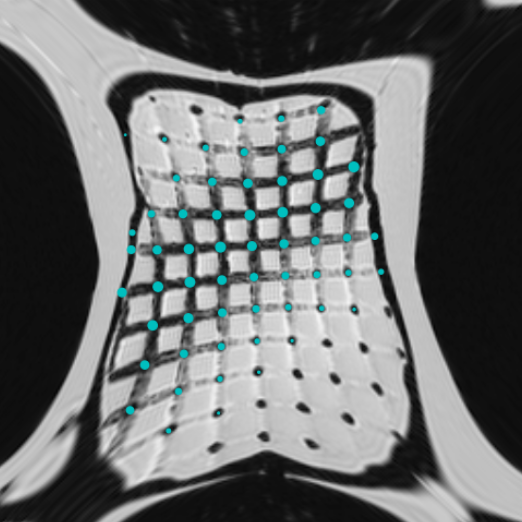
\includegraphics[width=\textwidth]{distorted-image.png}
        \caption{Distorted Image}
        \label{fig:test-case_2}
    \end{subfigure}
    \caption{Example test case with extreme distortion.  In order to validate our algorithms, we apply a known distortion to existing MRI source images.  Fiducials are manually identified on the source image, and are overlaid as light blue circles on the source image, (a).  The size of the circles indicates their position along the slice-axis (i.e. in or out of the page).  The circles overlaid on the distorted image, (b), are the points detected by one of our algorithms for this source image.}
    \label{fig:test-case}
\end{figure}

The final result of our testing framework is the mean target registration error, which is the mean value of the magnitude of the difference of the actual geometric distortion and the calculated geometric distortion \cite[page R37]{hill2001}.

\subsection*{Algorithm}

Our current algorithm combines our own ideas with those found in the literature (e.g. \cite{stanescu2010,baldwin2007}).  

Features are detected in the distorted image by convolving it with a 3D kernel shaped like the phantom grid intersections.  The convolved image tends to have peaks at the feature locations.  We threshold the convolved image and find the center of mass of regions of pixels centered at each peak.

At this point, we have a set of automatically calculated fiducials.  Next we need to apply a rigid registration (e.g. Figure \ref{fig:problem-overview}c) so that we can extract the geometric distortion from each pair of matching fiducials.  Performing this rigid registration precisely is complicated by a number of factors.

Not all of the fiducials will be correctly detected and there will be extra points that do not correspond to a real point.

The displacement between matching points has several components.  The geometric distortion introduced by the MRI is what we are attempting to measure, however there are other contributions to the displacement.  In particular, the first stage of our algorithm will likely introduce additional errors.

, which we denote as $B$, where $\forall \mathbf{b} \in B, \mathbf{b} \in \mathbb{R}^3$.

We denote the set of annotated fiducials as $A$ where $\forall \mathbf{a} \in A, \mathbf{a} \in \mathbb{R}^3$.



After detecting 

\section*{Results}

\section*{Discussion}

\bibliographystyle{ieeetr}
\bibliography{./algorithm.bib}

\end{document}
